\quad \quad The overall structure of the software system contains three layers: Student Management 
System, DataBase, and Queue Display System. The Student Management System is user end 
system which is related to administrative functionality that includes adding, removing 
and editing student and staff information in the system. The GUI allows the admin to 
add student and remove student. The DataBase System is responsible for storing the 
information. It also allows the user to make queries. The Queue Display System displays 
the information of the system and also handles the RFID listener. This is a user end 
system and also includes hardware. The Queue Display System and Database System 
communicate with each other to keep real time records of the student pickup.

\begin{figure}[h!]
	\centering
 	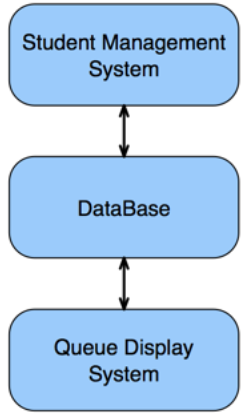
\includegraphics[width=0.40\textwidth]{images/ads_1}
 \caption{Overall Structure of System}
\end{figure}

\subsection{Student Management System Layer Description}
\quad \quad The Student Management System includes a control system, database control, and GUI. 
Control. This System directly talks with the Database System in order to store all the 
information about the students.

\subsection{Database Layer Description}
\quad \quad This System contains the tables to store the text and image of the system. Database 
System directly talks with Student Management System and Queue Display System.

\subsection{Queue Display System Layer Description}
\quad \quad This System contains control system, dbcontrol, GUI and RFID API. The RFID API helps 
to maintain communication between the Queue Display System and the RFID reader. The 
GUI displays the list of the students as their parents approach the school.